\documentclass[a4paper,11pt]{article}

\usepackage[utf8]{inputenc}
\usepackage[T1]{fontenc}
\usepackage[french]{babel}
% \usepackage{fullpage}
\usepackage{amsmath, amsfonts, amssymb, amsthm}
% \usepackage{mathabx}
% \usepackage{bbm}
\usepackage{stmaryrd}
\usepackage{graphicx}
% \usepackage{enumerate}

\usepackage{subfigure}
\usepackage{float}

% notations textuelles condensées
	\newcommand{\ssi}{si, et seulement si, }
	\newcommand{\ps}{\ensuremath{\text{ p.s.}}}



% restriction d'applications
	\newcommand{\restrictionaux}[2]{{#1\,\smash{\vrule height .8\ht1 depth .85\dp1}}_{\,#2}}
	\newcommand{\restr}[2]{\ensuremath{\mathchoice
		{\setbox1\hbox{${\displaystyle #1}_{\scriptstyle #2}$}
		\restrictionaux{#1}{#2}}
		{\setbox1\hbox{${\textstyle #1}_{\scriptstyle #2}$}
		\restrictionaux{#1}{#2}}
		{\setbox1\hbox{${\scriptstyle #1}_{\scriptscriptstyle #2}$}
		\restrictionaux{#1}{#2}}
		{\setbox1\hbox{${\scriptscriptstyle #1}_{\scriptscriptstyle #2}$}
		\restrictionaux{#1}{#2}}}}



% notations mathématiques
	% applications
		\newcommand{\map}[4]{\ensuremath{\begin{array}{r c l}#1&\to&#2\\#3&\mapsto&#4\end{array}}}
		\newcommand{\mapp}[6]{\ensuremath{\begin{array}{r c l}#1&\to&#2\\#3&\mapsto&#4\\#5&\mapsto&#6\end{array}}}

	% listes d'éléments
		\newcommand{\set}[1]{\ensuremath{\left\lbrace #1 \right\rbrace}}
		\newcommand{\scal}[2]{\ensuremath{\left<#1,#2\right>}}
		\newcommand{\couple}[2]{\ensuremath{\left(#1,#2\right)}}
		\newcommand{\seq}[2]{\ensuremath{\displaystyle{\left(#1\right)_{#2}}}}

	% notations d'Euler
		\newcommand{\integrale}[2]{\ensuremath{\displaystyle{\int_{#1}^{#2}}}}
		\newcommand{\somme}[2]{\ensuremath{\displaystyle{\sum_{#1}^{#2}}}}
		\newcommand{\produit}[2]{\ensuremath{\displaystyle{\prod_{#1}^{#2}}}}
		\newcommand{\union}[2]{\ensuremath{\displaystyle{\bigcup_{#1}^{#2}}}}
		\newcommand{\inter}[2]{\ensuremath{\displaystyle{\bigcap_{#1}^{#2}}}}
		\newcommand{\sommedirecte}[2]{\ensuremath{\displaystyle{\bigoplus_{#1}^{#2}}}}
		\newcommand{\tensoriel}[2]{\ensuremath{\displaystyle{\bigotimes_{#1}^{#2}}}}
		\newcommand{\cartesien}[2]{\ensuremath{\displaystyle{\bigtimes_{#1}^{#2}}}}

	% normes
		\newcommand{\abs}[1]{\ensuremath{\left| #1 \right|}}
		\newcommand{\norm}[1]{\ensuremath{\left\| #1 \right\|}}

	% probabilités
		\newcommand{\univers}{\ensuremath{\left(\Omega, \mathcal F, \mathbb P \right)}}
		\newcommand{\proba}[1]{\ensuremath{\mathbb P\left(#1\right)}}



% mise en forme
	\newcommand{\notion}{}



% préférences personnelles de typographie
	\renewcommand{\epsilon}{\varepsilon}
	% \renewcommand{\phi}{\varphi}
	\renewcommand{\tilde}{\widetilde}
	\renewcommand{\hat}{\widehat}
	\renewcommand{\bar}{\widebar}



% opérateurs mathématiques
	\DeclareMathOperator{\id}{id}
	\DeclareMathOperator{\Ran}{Im}
	\DeclareMathOperator{\Ker}{Ker}
	\DeclareMathOperator{\Tr}{Tr}
	\DeclareMathOperator{\supp}{supp}
	\DeclareMathOperator{\Vect}{Vect}
	\DeclareMathOperator{\pr}{pr}
	\DeclareMathOperator{\Int}{Int}
	%\DeclareMathOperator{\ln}{ln}



% théorèmes
	\theoremstyle{plain} %résultats
		\newtheorem{thm}{Théorème}[section]
		\newtheorem{cor}[thm]{Corollaire}
		\newtheorem{pte}[thm]{Propriété}
		\newtheorem{prop}[thm]{Proposition}
		\newtheorem{res}[thm]{Résultat}
		\newtheorem{lem}[thm]{Lemme}
	\theoremstyle{definition} %définitions
		\newtheorem{definition}[thm]{Définition}
	\theoremstyle{remark} %remarques
		\newtheorem*{rk}{Remarque}

\title{Projet de simulations aléatoires : Modèles d'Ising}
\author{Aurélien Enfroy, Shmuel Rakotonirina{-}-Ricquebourg}

\begin{document}
\maketitle
\tableofcontents

\section{Introduction}

Ce document rend compte d'expériences sur les modèles d'Ising sur un réseau carré, avec pour objectifs principaux d'observer la transition de phase à la température critique, en fonction de la taille du réseau. En théorie, à température sur-critique, les états les plus probables ont des spins assez mélangés, alors qu'à température sous-crituque, les états les plus probables rassemblent entre eux les spins identiques.

Nous avons fait le choix, pour s'approcher le mieux possible d'un réseau infini, de prendre des conditions aux bords périodiques (par exemple, les points du côté droit du carré sont voisins du côté gauche).

Pour l'observation de la température critique (réseau de grande taille), nous avons implémenté l'échantilloneur de Gibbs (section \ref{sec:gibbs}), l'algorithme de Metropolis-Hastings (section \ref{sec:MH}), et deux méthodes de couplage par le passé, chacune basée sur une des méthodes précédentes (section \ref{sec:coupling}). La section \ref{sec:check} présente la magnétisation et le test qui en découle pour vérifier que ces algorithmes fonctionnent.

En très petite taille (4 ou 9 sommets sur le graphe), nous avons aussi implémenté la méthode naïve (section \ref{sec:naive}) pour observer à quel point les états $\pm(1,\hdots,1)$ étaient probable (et donc "résistants" aux transitions de Metropolis-Hastings).

Enfin, la section \ref{sec:tc} présente les observations des transitions de phase autour de la température critique théorique, pour différentes tailles de réseau.

\section{Choix d'implémentation}\label{sec:implementation}

On rappelle la définition du modèle d'Ising sur un réseau carré :
\begin{definition}
On fixe $C$ le réseau carré de dimension 2 de taille $N^2$. Le modèle d'Ising est la distribution sur l'espace d'état $\set{\pm 1}^C$ dont la loi est donnée par
$$\forall x \in \set{\pm 1}^C, \pi(x) = \frac{1}{Z_T} \exp \left(\left( \somme{u\sim v}{} J_{u,v} x_{u} x_{v} + \somme{u}{} h_{u} x_{u} \right)/T\right)$$
où $T>0$ est appelée la température, $Z_T$ est une constante de normalisation, $J_{u,v}$ est la force d'interaction entre $u$ et $v$ et $h_{u}$ est le champ magnétique extérieur en $u$.
\end{definition}

Pour l'implémentation, on remarque qu'il n'y a pas besoin du paramètre $T$, qu'on peut inclure dans $J$ et $h$. On représente alors ces paramètres en prenant $x \in \mathcal M_{N,N}(\set{\pm 1})$, $\tilde h = h/T \in \mathcal M_{N,N}(\mathbb R)$ et $J$ comme une matrice à trois entrées $\tilde J \in \mathcal M_{N,N,2}(\mathbb R)$ où
$$\tilde J_{i,j,1} = J_{(i,j),(i+1,j)}/T \text{ et } \tilde J_{i,j,2} = J_{(i,j),(i,j+1)}/T$$
où $i+1$ et $j+1$ sont à comprendre modulo $N$ pour obtenir des conditions aux bords périodiques.

Dans le but de créer le script \texttt{animations.sce} (qui montre en animation l'évolution des différentes chaînes), nous avons dû stocker de très grandes matrices (à $N^2n$ entrées, où $n$ est le temps d'évolution des chaînes). Cependant, le type par défaut \texttt{double} stocke les données sur beaucoup plus de bits que nécessaire, causant donc des erreurs d'allocation mémoire quand les chaînes mémorisées devenaient trop longues et les matrices trop grandes. Nous avons donc fait le choix de stocker tous les spins (donc toutes les variables ne pouvant prendre que les valeurs $\pm 1$) sur 8 bits (type \texttt{int8}, qui est le type pouvant stocker $\pm 1$ prenant le moins de mémoire), ce qui nécessite de changer des \texttt{double} en \texttt{int8} et réciproquement pour certains calculs (d'où l'apparition répétée dans nos codes des fonctions \texttt{double} et \texttt{int8}).

Il aurait été possible de prendre encore moins de mémoire en remplaçant les $\pm 1$ par des booléens \texttt{\%t} et \texttt{\%f}, en remplaçant donc les $*$ par des \texttt{xor}. Mais cela rendait le code moins lisible, notamment quand on voulait multiplier un booléen par un \texttt{double} (par exemple pour calculer $J_{u,v} x_{u} x_{v}$, où $J$ est stocké en \texttt{double} et $x$ en booléen). De plus, nous n'avons pas eu de problème mémoire avec le type \texttt{int8}, il n'a donc pas été nécessaire de faire plus d'économie.

\section{Simulation par l'échantilloneur de Gibbs}\label{sec:gibbs}

En reprenant les notations du cours, on a pour $u \in C$ et $x \in \set{\pm 1}^C$, les transitions coordonnées par coordonnées suivantes
\begin{align*}
\pi_u(x_u \mid x^u)
&= \frac{\pi(x_u,x^u)}{\pi(1,x^u) + \pi(-1,x^u)}\\
&= \frac{e^{x_u V_u(x)}}{e^{V_u(x)} + e^{-V_u(x)}}
\end{align*}
où on note encore $V_u(x) \doteq \left( \somme{v \sim u}{} J_{u,v} x_v + h_u \right) /T$. Donc $\pi_u(\cdot \mid x^u) = \mathcal B(\frac{e^{V_u(x)}}{e^{V_u(x)} + e^{-V_u(x)}}) = B(\frac{1}{1 + e^{-2V_u(x)}})$. L'échantillonneur de Gibbs consiste à actualiser une entrée de la matrice en laissant inchangé le reste de la matrice et en donnant à cette entrée un spin tiré selon la loi $\pi_u(\cdot \mid x^u)$.

Nous avons implémenté ici les deux versions de l'échantillonneur de Gibbs :
\begin{itemize}
	\item Le balayage séquentiel : à chaque itération de l'algorithme, on actualise toutes les entrées, dans un ordre fixé.
	\item Le balayage aléatoire : à chaque itération de l'algorithme, on ne modifie qu'une entrée, choisie uniformément sur tout le réseau.
\end{itemize}
Pour obtenir des temps d'exécutions similaires, et pour équilibrer les vitesses à laquelle les algorithmes convergent, pour chaque itération de l'échantillonneur de Gibbs à balayage séquentiel, on effectue $N^2$ itérations de celui aléatoire.

\section{Simulation par Metropolis-Hastings}\label{sec:MH}

Nous avons implémenté l'algorithme de Metropolis-Hastings en utilisant la fonction de rejet de Metropolis-Hastings. Pour le choix du noyau instrumental $Q$, nous avons choisi de donner à une coordonnée aléatoire (uniforme) une valeur aléatoire (uniforme), ce qui permet d'avoir un noyau symétrique irréductible apériodique (probabilité strictement positive de rester sur place).

Avec ce noyau instrumental, on peut réduire les calculs effectués : si $x$ est un état et $y$ l'état proposé à partir de $x$, alors
\begin{itemize}
	\item soit $y = x$, auquel cas on peut considérer qu'on accepte le mouvement,
	\item soit $y \neq x$, auquel cas ils ne diffèrent que d'au plus une coordonnée (celle tirée uniformément). Si on note $u$ cette coordonnée et $s$ la nouvelle valeur, alors $s = y_u = - x_u$ et, en considérant que $T$ a été pris en compte dans $J$ et $h$,
	\begin{align*}
	\frac{\pi(y)}{\pi(x)}
	&= \frac{\exp \left(\left( \somme{v \sim u}{} J_{u,v} s x_{v} + h_{u} s \right) /T \right)}{\exp \left(\left( \somme{v \sim u}{} J_{u,v} (-s) x_{v} + h_{u} (-s) \right) /T \right)}\\
	&= \frac{e^{s V_u(x)}}{e^{-s V_u(x)}}\\
	&= e^{2 s V_u(x)}
	\end{align*}
	où on a noté $V_u(x) \doteq \left( \somme{v \sim u}{} J_{u,v} x_v + h_u \right) /T$.
\end{itemize}

Dans le cas de l'échantillonneur de Gibbs et de Metropolis-Hastings, le temps passé pour les actualisations est presque entièrement dû aux calculs des $V_u(x)$ et des exponentielles. Cette disjonction de cas donne donc un avantage à l'algorithme de Metropolis-Hastings sur l'échantillonneur de Gibbs : dans la moitié des cas, il n'y a pas de calcul à faire pour Metropolis-Hastings. Cela se traduit par un temps d'exécution deux fois plus court en moyenne pour Metropolis-Hastings.

\section{Couplage par le passé}\label{sec:coupling}

Pour le couplage par le passé, deux fonctions d'actualisation sont possibles. 
\begin{itemize}
	\item celle vue en cours, issue de l'échantillonneur de Gibbs (par balayage séquentiel)
	\item celle de \cite{propp1998coupling}, issue de l'algorithme de Metropolis-Hastings (i.e. même transition qu'en section \ref{sec:MH}).
\end{itemize}
Dans les deux cas, la méthode n'a de garantie théorique que si $J$ est constant et $h$ nul. On supposera donc cela vérifié.

L'algorithme consiste à répéter les algorithmes (Metropolis Hastings ou échantilloneur de Gibbs), vers le futur, en partant des états $\pm(1,\hdots,1)$  jusqu'à un temps fixé à l'avance. Si il n'y a pas eu coalition, on ajoute des nouvelles actualisations au début du processus (en conservant les actualisations précédentes à la fin du processus), ce qui demande de recalculer le processus dans son entièreté. Pour obtenir le temps de coalition exact, il faudrait en théorie n'ajouter qu'une actualisation à la fois. Cependant, on ne cherche pas à obtenir ce temps, on se contente donc de doubler le nombre d'actualisations à chaque échec de coalition.

Pour les deux méthodes (Metropolis-Hastings et échantillonneur de Gibbs), les choses se passent bien au-delà de la température critique. Cependant, à (très) basse température, les états $\pm(1,\hdots,1)$ sont très probables et ont donc tendance à rester inchangés par les fonctions d'actualisation précédentes : dans les deux cas, la probabilité de réussir à changer un point $x_u$ égaux à ses quatre voisins est très faible : si $J>0$ (toujours supposé constant), alors elle vaut $\exp(-8 J/T)$.

En conséquence, l'algorithme met extrêmement longtemps à terminer (nous ne l'avons pas vu terminer) quand la température est trop basse (par rapport à la température critique). En observant l'évolution des chaînes de Markov démarrant de $(1,\hdots,1)$ et de $(-1,\hdots,-1)$, on voit que souvent les deux chaînes reviennent à leur état initial, ce qui signifie que l'algorithme pourrait bien continuer de boucler ainsi très longtemps. À titre d'exemple, à $T = 2.2$ (sous-critique mais proche de la température critique) et $N = 50$ (donc $2500$ entrées par matrices), on peut noter $e$ le nombre d'entrées par lequel les deux chaînes diffèrent encore après $n$ actualisation de type Metropolis-Hastings, ce qui donne les tables \ref{tab:non_coalition}. Plus généralement, quand $T$ augmente, on a besoin de moins en moins d'actualisations.
\begin{table}[!htbp]
	\label{tab:non_coalition}
	\centering
	\hfill
	\subfigure[Cas sous-critique $T = 2.2$ (interrompu au bout de $\sim 1500s$)]{
		\begin{tabular}{c|c}
			$n$ & $e$ \\
			\hline \hline
			$2500$ & $2434$ \\
			\hline
			$5000$ & $2408$ \\
			\hline
			$10000$ & $2353$ \\
			\hline
			$20000$ & $2272$ \\
			\hline
			$40000$ & $2189$ \\
			\hline
			$80000$ & $2130$ \\
			\hline
			$160000$ & $2088$ \\
			\hline
			$320000$ & $2066$ \\
			\hline
			$640000$ & $2066$ \\
			\hline
			$1280000$ & $2066$
		\end{tabular}
	}
	\hfill
	\subfigure[Cas sur-critique $T = 3$]{
		\begin{tabular}{c|c}
			$n$ & $e$ \\
			\hline \hline
			$2500$ & $2331$ \\
			\hline
			$5000$ & $2193$ \\
			\hline
			$10000$ & $1965$ \\
			\hline
			$20000$ & $1573$ \\
			\hline
			$40000$ & $1028$ \\
			\hline
			$80000$ & $567$ \\
			\hline
			$160000$ & $103$ \\
			\hline
			$320000$ & $0$
		\end{tabular}
	}
	\hfill
	\caption{Tentatives de coalition consécutives de l'algorithme de couplage par le passé par Metropolis-Hastings. Pour passer de $n$ à $2n$, on conserve les $n$ actualisation et on en ajoute $n$ nouvelles avant. $e$ est le nombre d'entrées différentes entre les deux chaînes à la fin de la tentative à $n$ fixé ($e \leq N^2 = 2500$, il y a coalition à $e = 0$)}
\end{table}

Pour cette raison, on préfèrera à cet algorithme les algorithmes précédant, non exacts mais pour lequels on peut décider à l'avance du temps utilisé par l'algorithme.

On vérifie quand même que les comportements des différents algorithmes sont similaires au cas sans couplage figure \ref{fig:compar_vis}, avec des temps d'exécution donnés figure \ref{tab:compar_tps}. On indique le nombre d'actualisations calculées (appelées \emph{transitions} en figure \ref{fig:compar_vis}) à côté du temps.
\begin{rk}

\begin{itemize}
	\item Chaque balayage séquentiel coûte $N^2$ actualisations. Donc en figure \ref{fig:compar_vis}, 100 balayages séquentiels correspondent à 250000 transitions.
	\item Pour les algorithmes de couplage, environ la moitié des actualisations calculées sont utiles. Les autres ont été oubliées après n'avoir pas conduit à une coalition. Par exemple, à $T = 5$ avec Metropolis-Hastings, $80000$ actualisations sont utiles, mais l'algorithme a fait $N^2 = 2500$ actualisations, puis $5000$, $10000$, $20000$, $40000$, chaque fois sans qu'il y ait coalition, puis $80000$ où il y a eu coalition, d'où un total de $157500$ actualisations calculées.
\end{itemize}
\end{rk}
\begin{figure}[!htbp]
	\centering
	\subfigure[$T = 3$]{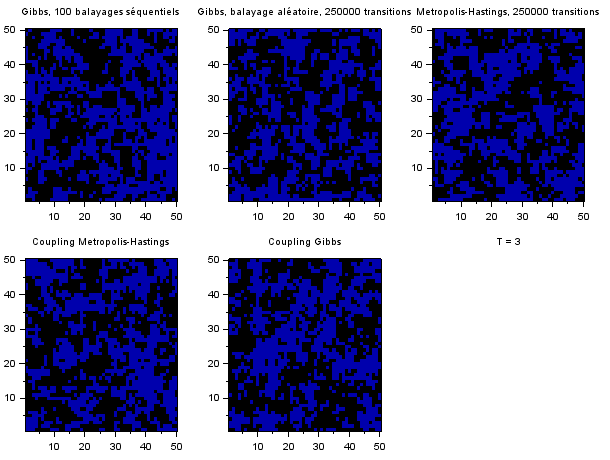
\includegraphics[width=\textwidth]{comparaison_N50_n100_T3.png}}
	\subfigure[$T = 5$]{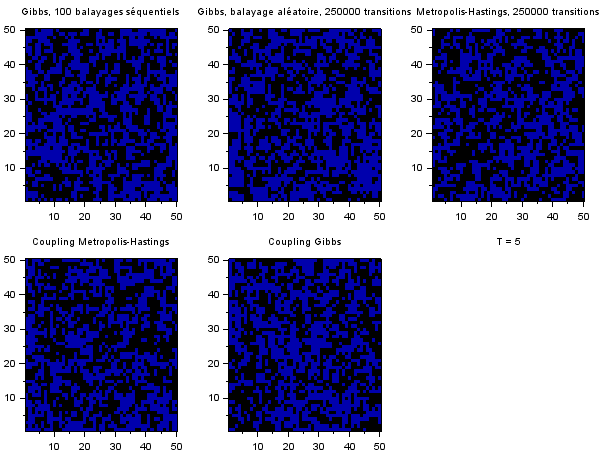
\includegraphics[width=\textwidth]{comparaison_N50_n100_T5.png}}
	\caption{Comparaison visuelle de résultats des algorithmes}
	\label{fig:compar_vis}
\end{figure}
\begin{table}[!htbp]
	\centering
	\begin{tabular}{r|||c||c|}
		Méthode & $T = 3$ & $T = 5$ \\
		\hline \hline
		Gibbs séquentiel & 209s [250 000] & 209s [250 000] \\
		\hline
		Gibbs aléatoire & 209s [250 000] & 208s [250 000] \\
		\hline
		Metropolis-Hastings & 115s [250 000] & 98s [250 000] \\
		\hline
		Couplage Metropolis-Hastings & 520s [637 500] & 115s [157 500] \\
		\hline
		Couplage Gibbs séquentiel & 532s [317 500] & 118s [77 500]
	\end{tabular}
	\caption{Comparaison des temps d'exécution des algorithmes pour $N = 50$. Entre crochets le nombre d'actualisations calculées}
	\label{tab:compar_tps}
\end{table}
Les résultats des algorithmes sont bien similaires pour différentes températures (sur-critiques), et à nombre d'actualisation fixée, on vérifie bien que l'algorithme de Metropolis-Hastings est deux fois plus rapide.

\section{Vérification des algorithmes}\label{sec:check}

Pour vérifier que les algorithmes MCMC fonctionnent, on utilise la fonction $M(x) = \frac{1}{N^2} \sum_u x_u$. $M$ est appelée la magnétisation. Dans le cas où $h = 0$, on a $\pi(-x) = \pi(x)$ et $M(-x) = -M(x)$ donc si $X \sim \pi$, alors $\mathbb E(M(X)) = 0$. Or la chaîne $(X^{(n)})_n$ (ici $(X^{(n)})_n$ représente la chaîne de Markov pour Metropilis Hastings ou gibbs) est ergodique, car c'est une chaîne de Markov à espace d'etats fini, irréductible et aperiodique. On aura donc la convergence presque sûre:
$$\frac{1}{n} \sum_i M(X^{(i)}) \xrightarrow[n \rightarrow +\infty]{} \displaystyle \int_{}^{} M(x) \, \mathrm{d}\pi(x)=\mathbb E(M(X)) = 0$$
En pratique, à basse température, les algorithmes ont tendance à rester longtemps dans les états $(1,\hdots,1)$ et $(-1,\hdots,-1)$ (qui sont très probables à basse température) donc il faudrait attendre un temps très long pour voir cette convergence. On se place donc à haute température.

Pour l'algorithme exact (couplage par le passé), on simule de manière indépendante un échantillon $(X^{(n)})_n$ et on vérifie que la loi des grands nombres s'applique :
$$\frac{1}{n} \sum_i M(X^{(i)}) \xrightarrow[n \rightarrow +\infty]{} \mathbb E(M(X)) = 0.$$

On obtient les résultats de la figure \ref{fig:ergodic}.
\begin{figure}[!htbp]
	\centering
	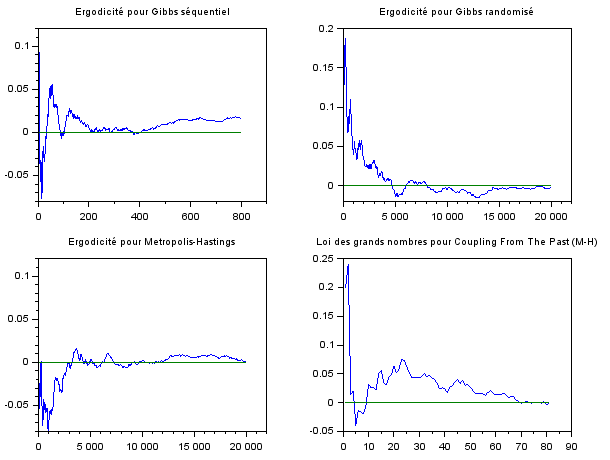
\includegraphics[width=0.8\textwidth]{ergodicite_magnetisation.png}
	\caption{Vérification de l'ergodicité et de la loi des grands nombres sur la magnétisation}
	\label{fig:ergodic}
\end{figure}

\section{Cas en petite taille : simulation naïve et température critique}\label{sec:naive}

En petite taille, on peut faire une simulation naïve. Pour cela, on numérote les $2^{N^2}$ états (dans l'ordre lexicographique en lisant les matrices colonne par colonne), on calcule exactement la loi et on choisit un numéro en utilisant cette loi et une loi uniforme sur $[0,1]$.

On a donc une représentation (dans un vecteur \texttt{p} dans le code SciLab) de toutes les probabilités de tous les états, et des fonctions (\texttt{etat2num} et \texttt{num2etat}) qui associent une matrice $x \in \set{\pm 1}^C$ à sa numérotation $m \in \llbracket 1,2^{N^2} \rrbracket$ ou une numérotation à sa matrice.

Le calcul des probabilités exactes permet de tracer, en fonction de $T$, la probabilité d'un état donné. La figure \ref{fig:tc_naive_N4} trace la probabilité de l'état $(1,\hdots,1)$ (qui est celle de $(-1,\hdots,-1)$).
\begin{figure}[!htbp]
	\centering
	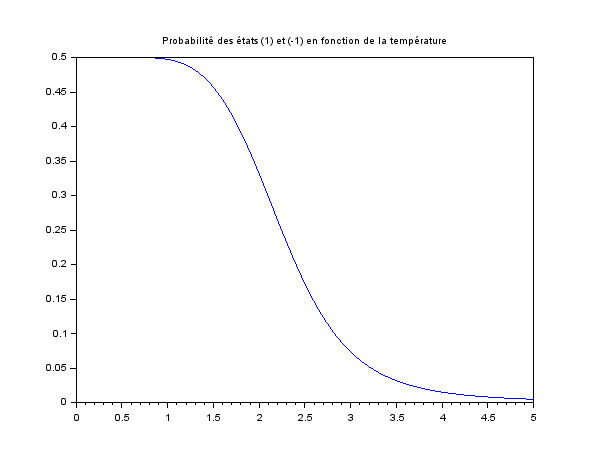
\includegraphics[width=0.8\textwidth]{temperature_critique_naive_N4.png}
	\caption{$\pi(1,\hdots,1)$ en fonction de $T$ pour $N = 4$}
	\label{fig:tc_naive_N4}
\end{figure}
On observe une décroissance assez lente autour d'une température critique inférieure à la température critique théorique $T_c \simeq 2.269$. La théorie dit que quand $N \rightarrow +\infty$, cette décroissance devient de plus en plus forte et de plus en plus concentrée autour de $T_c$. En effet, les spins différents ont plus de chance de coexister en haute température, les états avec un spin majoritaire sont donc moins probables.

\section{Observation de la transition de phase selon la taille du réseau}\label{sec:tc}

Comme dit en section \ref{sec:naive}, en très petite taille, la température critique est en dessous de la température critique théorique. On s'attend donc qu'avec l'augmentation de la taille du réseau, la température critique augmente en tendant vers la température critique théorique.

Un inconvénient pour observer cela est qu'en petite taille, il peut être difficile de distingué une température sous-critique et une sur-critique, sauf quand elles sont loin de la température critique, en témoigne la figure \ref{fig:tc_gibbs_N20_n25}.
\begin{figure}[!htbp]
	\centering
	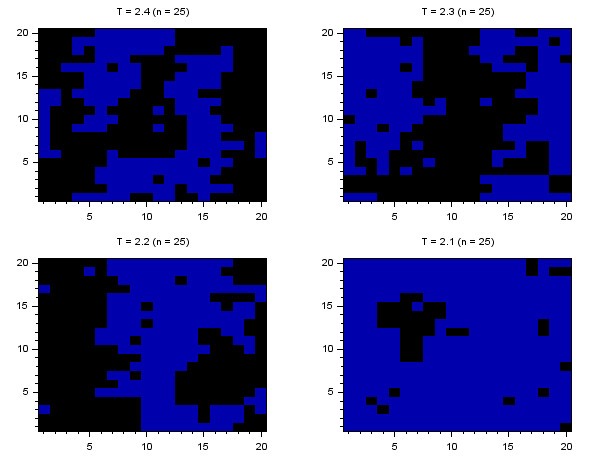
\includegraphics[width=0.8\textwidth]{temperature_critique_gibbs_N20_n25.png}
	\caption{Simulation par échantillonneur de Gibbs ($n = 25$ balayages séquentiels), $N = 20$}
	\label{fig:tc_gibbs_N20_n25}
\end{figure}
On y voit une différence claire de comportement entre $T = 2.1$ (où les spins sont peu mélangés) et les températures supérieures, mais les motifs observés sont trop petits pour distinguer des différences entre les autres configurations. La température critique effective semble alors se situer entre $2.1$ et $2.2$.

En augmentant la taille du réseau (figure \ref{fig:tc_gibbs_N50_n25}), on distingue mieux les comportements différents.
\begin{figure}[!htbp]
	\centering
	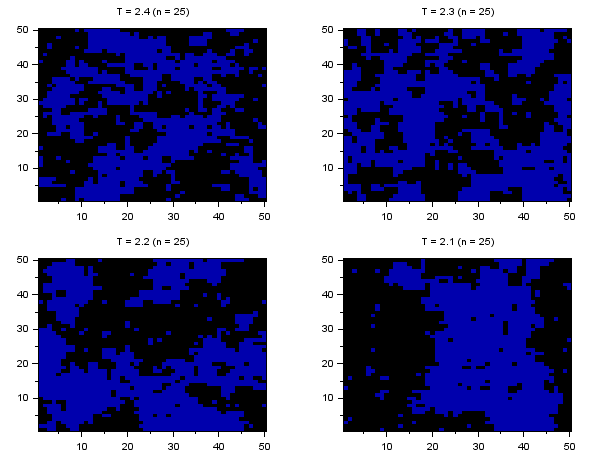
\includegraphics[width=0.8\textwidth]{temperature_critique_gibbs_N50_n25.png}
	\caption{Simulation par échantillonneur de Gibbs ($n = 25$ balayages séquentiels), $N = 50$}
	\label{fig:tc_gibbs_N50_n25}
\end{figure}
\begin{itemize}
	\item À $T = 2.1$, on distingue très clairement deux blocs de spins (les conditions aux bords étant périodiques, le bloc de droite composé de $-1$ (noir) est en contact avec le bord noir de gauche, tout comme les côtés noir haut et bas coïncident). La température est donc trop basse pour que les spins différents se mélangent, au point où les états probablent rassemblent les spins identiques en un unique bloc.
	\item À $T = 2.2$, il n'y a toujours que deux blocs mais le comportement est plus proche de celui observé en figure \ref{fig:tc_gibbs_N20_n25} : ces blocs ne sont pas aussi nettement délimités qu'à $T = 2.1$ et sont intriqués l'un dans l'autre.
	\item À $T \geq 2.3$, il commence à y avoir un mélange des différents spins, même si localement les spins identiques sont rassemblés en blocs. On observe ainsi de nombreux blocs, ainsi que des spins isolés, et il y en a d'autant plus que $T$ augmente.
\end{itemize}
Ces observations poussent à placer la température critique entre $2.2$ et $2.3$ mais un autre comportement est possible (figure \ref{fig:tc_gibbs_N50_n50}).
\begin{figure}[!htbp]
	\centering
	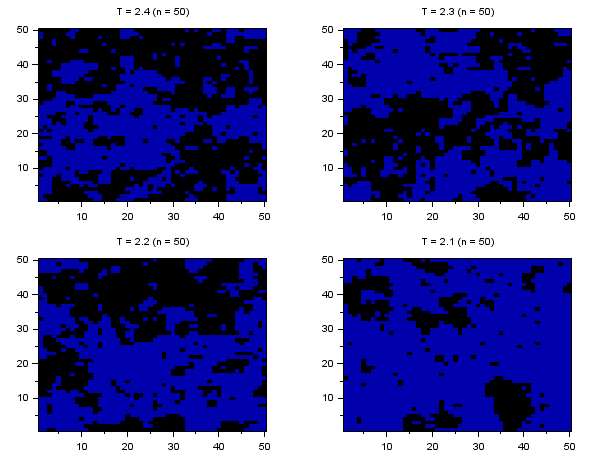
\includegraphics[width=0.8\textwidth]{temperature_critique_gibbs_N50_n50.png}
	\caption{Simulation par échantillonneur de Gibbs ($n = 50$ balayages séquentiels), $N = 50$}
	\label{fig:tc_gibbs_N50_n50}
\end{figure}
Ici, les comportements à $T \geq 2.2$ sont assez similaires à précédemment (des blocs de spins et des spins isolés, avec des blocs d'autant plus petit et des spins isolés d'autant plus nombreux que la température est haute), mais la différence entre $T = 2.3$ et $T = 2.2$ n'est plus aussi nette. Au contraire, à $T = 2.1$ on observe un état avec très peu de spins $-1$, rassemblés en petit blocs plongés dans une majorité de spin $+1$. C'est un comportement attendu sous la température critique (une majorité d'un spin donné), on pourrait donc placer la température critique entre $2.1$ et $2.2$.

En augmentant encore la taille du réseau, la transition de phase est beaucoup plus évidente, même en temps court (figure \ref{fig:tc_gibbs_N100_n25}).
\begin{figure}[!htbp]
	\centering
	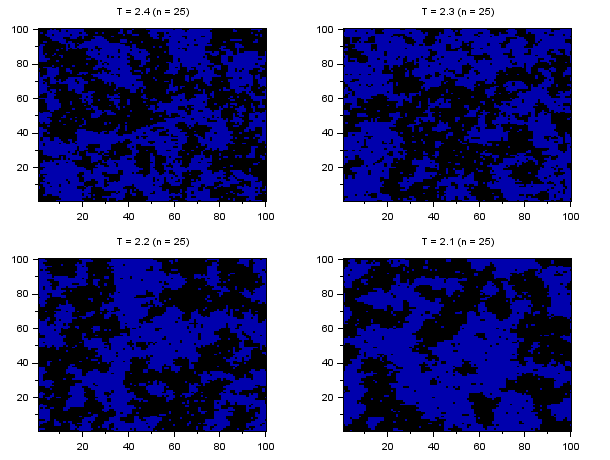
\includegraphics[width=0.8\textwidth]{temperature_critique_gibbs_N100_n25.png}
	\caption{Simulation par échantillonneur de Gibbs ($n = 25$ balayages séquentiels), $N = 100$}
	\label{fig:tc_gibbs_N100_n25}
\end{figure}
On peut ici séparer les quatre figures en deux groupes assez distincts :
\begin{itemize}
	\item un groupe $T \leq 2.2$, où des blocs bien délimités sont formés. La majorité des blocs formés sont de grande taille, et les spins isolés ou les blocs de petite taille sont peu nombreux et loin des frontières des blocs macroscopiques, participant à définir plus nettement les délimitations. Les blocs macroscopiques sont aussi connectés entre eux (par des "couloirs" ou des blocs microscopiques).
	\item un groupe $T \geq 2.3$, où les blocs n'ont pas de frontières précises, et chaque bloc d'un spin donné contient de nombreux spins opposés isolés. Il y a aussi beaucoup de blocs de petites tailles qui "contaminent" les blocs de grande taille, causant ce flou sur les frontières (et donc sur la définition) des blocs macroscopiques. Les blocs macroscopiques étant plus petits et plus flous que précédemment, ils ne sont pas ou peu connectés entre eux.
\end{itemize}
Le comportement est identique (et d'autant plus marqué) quand on laisse l'algorithme tourner plus longtemps (figures \ref{fig:tc_gibbs_N100_n50} et \ref{fig:tc_MH_N100_n100}).
\begin{figure}[!htbp]
	\centering
	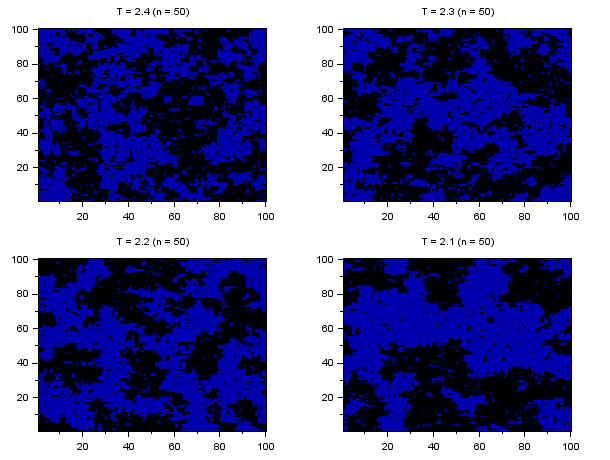
\includegraphics[width=0.8\textwidth]{temperature_critique_gibbs_N100_n50.png}
	\caption{Simulation par échantillonneur de Gibbs ($n = 50$ balayages séquentiels), $N = 100$}
	\label{fig:tc_gibbs_N100_n50}
\end{figure}
\begin{figure}[!htbp]
	\centering
	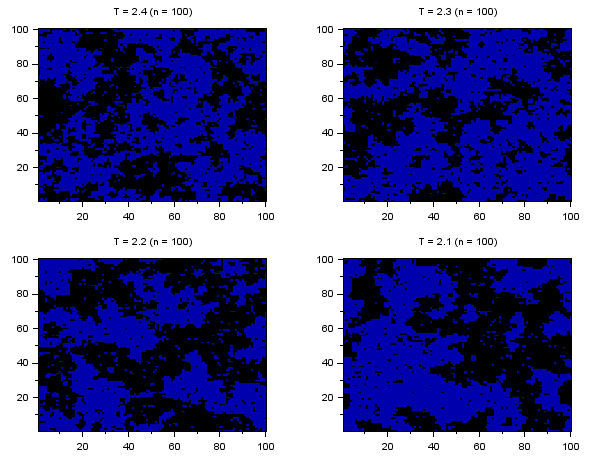
\includegraphics[width=0.8\textwidth]{temperature_critique_MH_N100_n100.png}
	\caption{Simulation par Metropolis-Hastings ($nN^2 = 500000$ actualisations), $N = 100$}
	\label{fig:tc_MH_N100_n100}
\end{figure}
Les figures \ref{fig:tc_gibbs_N100_n25}, \ref{fig:tc_gibbs_N100_n50} et \ref{fig:tc_MH_N100_n100} donnent donc une température critique entre $2.2$ et $2.3$, ce qui correspond bien à la température critique théorique ($\simeq 2.27$).

\section{Conclusion}

À $J = 1$ et $h = 0$, on dispose d'une méthode exacte (couplage par le passé par Metropolis-Hastings ou par échantillonneur de Gibbs) mais qui peut être très longue, notamment pour les températures sous-critiques et pour les réseaux de grande taille ; la durée d'exécution de cet algorithme n'est contrôlée qu'en espérance, ce qui empêche de les utiliser efficacement en pratique. En revanche, les algorithmes approchés (Metropolis-Hastings et échantillonneur de Gibbs, le premier étant plus rapide que le second) permettent d'observer la transition de phase et l'influence de la taille du réseau sur celle-ci : les expériences ont bien confirmé que la température critique s'observait d'autant mieux que le réseau était grand, et qu'elle tendait de manière croissante vers la température critique théorique $T_c \simeq 2.269$.





\nocite{*}
\bibliographystyle{plain}
\bibliography{biblio}

\end{document}
